\documentclass[../../main.tex]{subfiles}

\begin{document}
    Zum Abschluss der Untersuchungen widmen wir uns der Abhängigkeit der Ausgabeleitung $P_{\textit{Nd:YAG}}$ von der Pumpleistung $P_{\textit{pump}}$ unter Einfluss eines nichtlinearen Kristalls. Dabei sind die Messdaten in Abbildung \ref{fig:PumpLaserLeistung} zu sehen. Wir fitten an diese eine quadratische Funktion der Form
    \[
        q_{a,b,c}(x) := a\cdot (x - b)^2 + c,
    \]
    wobei wir uns an den theoretischen Zusammenhang der Fundamentalwelle zur frequenzverdoppelten Welle und der Leistungsbeziehung $P_{w\nu}(P_\nu) = k\cdot P_\nu^2$ mit entsprechender Proportionalitätskonstante $k$. Dabei nutzen wir die eingeführte Verschiebung zur direkten Ermittlung des Lasingpunktes vom Nd:YAG Laser \cite[p. 19]{doc:experiment08}. Damit erhalten wir den $b$ Verschiebungsparameter wie in Tabelle \ref{tab:PumpLaserLeistungFitParameter} dargestellt.
    \begin{figure}[H]
        \centering
        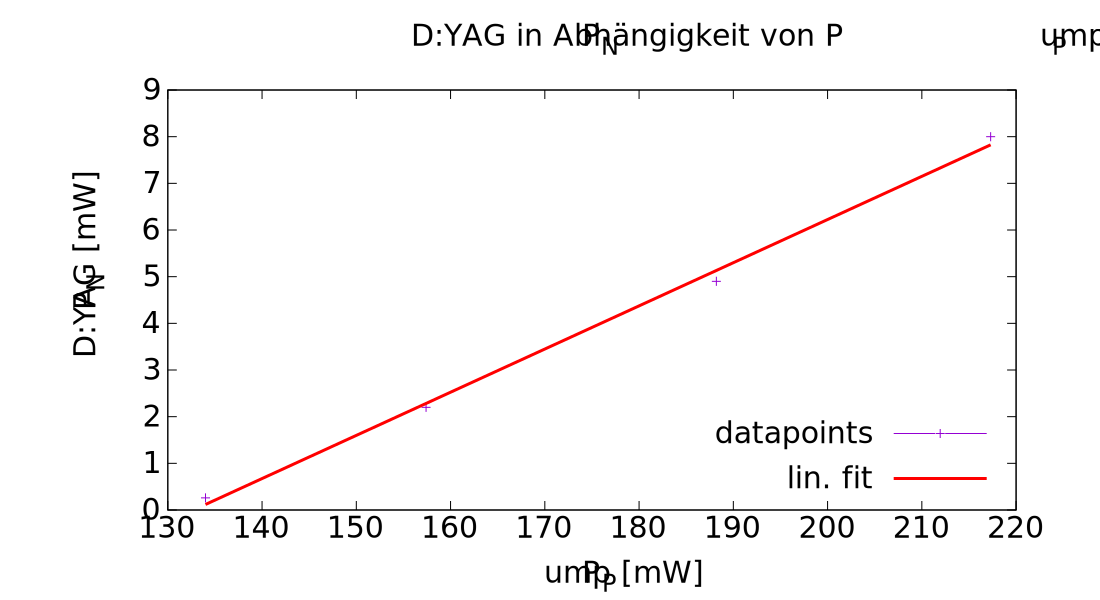
\includegraphics[width=11cm]{../../Bilddateien/7-2/P(NDYAG)overP(Pump).png}
        \caption{Die Laserleistung $P_{\textit{Nd:YAG}}$ als Funktion der Pumpleistung $P_{\textit{pump}}$}
        \label{fig:PumpLaserLeistung}
    \end{figure}
    \begin{table}[H]
        \centering
        \begin{tabular}{c|cc}
            \hline
             & $b$ in $\si{\mW}$ & $u(b)$ in $\si{\mW}$ \\
            \hline\hline
            $q_{a, b, c}$ & $110.833$ & $20.78$
        \end{tabular}
        \caption{Die Parameter der quadratischen Kurvenanpassung.}
        \label{tab:PumpLaserLeistungFitParameter}
    \end{table}
    Die Charakterisierung über die $RSS$ liefert uns den Wert $RSS(q_{a,b,c}) = 4.79107$.\\

    Durch das frequenzverdoppelte Licht theoretisch sichtbare Lichtmoden im Resonator konnten nicht beobachtet werden.
\end{document}